\section{Applications {\bf{(Reik + Jonathan)}}}\label{sec:Applications}
In this section, we illustrate the application of the above discussed methods on selected examples from theory and real-world research questions. We focus on recurrence network approaches, (horizontal) visibility graphs, and transition network approaches since those methods have found a much wider and deeper applications in diverse research fields. 

% RVD: My understanding of this section was rather that we collect information on all recent applications of the different methods, instead of focusing on one or two per method. Shouldn't we rather have a separate section highlighting some results for well-studied model systems (logistic map, R\"ossler, Lorenz, etc.) using all different methods, instead of having too detailed discussions of certain real-world examples?

% (Update 15/02/17): I suggest splitting this section into two: (1) Numerical Examples, (2) Real-world applications. With that, we can easily proceed.

	\subsection{Recurrence networks}
	We separate this section in two subsections, corresponding to numerical examples and real-world applications respectively. 	
		\subsubsection{Numerical examples}
		\emph{Illustration of network properties in phase space: } 
		RN approaches can be useful for disentangling different dynamical regimes not only in dissipative, but also in Hamiltonian systems. For dissipative systems, characteristics based on recurrence networks have recently attracted much interest for discriminating qualitatively different types of dynamics in terms of measures of complexity, dynamical invariants, or even structural characteristics of the underlying attractor's geometry in phase space. More specifically, local vertex-wise network characteristics of time series can be visualized in the corresponding phase space \cite{Donner2010a}. For instance, phase spaces of discrete H\'enon map, the chaotic R\"ossler and Lorenz system have been color coded by vertex degrees $k$, local clustering coefficient $\mathcal{C}_v$ and betweenness $b_v$, respectively \cite{Donner2010a}. Furthermore, global network measures of transitivity $\mathcal{T}$, average path length $\mathcal{L}$ have been applied to identify dynamical transitions in the Logistic map when the control parameter is changed \cite{Marwan2009}.   
		
		In \cite{Zou2016d}, we demonstrate that the validity of the RN approach for achieving the same goals in low-dimensional Hamiltonian systems. Using the standard map as a paradigmatic example, we perform recurrence network analysis for distinguishing regular and chaotic orbits co-existing in the same phase space. Specifically, we show that sticky orbits of the standard map can have a distinct geometric organization that can be detected reliably by recurrence network analysis of relatively short time series (e.g., $N=1,000$ or $5,000$ points). Let us restrict our attention to the standard map
\begin{equation} \label{std_map_book}
\mathbf{v}(t): \left \{ \begin{aligned}
& y_{n+1} = y_{n} + \frac{\kappa}{2 \pi}\sin(2 \pi x_{n}),  \\
& x_{n+1} = x_{n} + y_{n+1},
\end{aligned} \;\;\text{mod}\;\; 1
\right.
\end{equation}
with $\kappa $ denoting the system's single control parameter, and $\mathbf{v}_n=(x_n,y_n)$ being the state vector of the system at its $n$-th iteration. This model is probably the best-studied chaotic Hamiltonian map and can be interpreted as a Poincar\'e section of a periodically kicked rotor \cite{Lichtenberg_Lieberman_regular,Meiss_rmp_1992}.
		
		The whole phase space presents a complicated mixture of domains of chaotic trajectories coexisting with domains of regular ones. The regular component consists of both periodic and quasi-periodic trajectories, while the irregular one contains one or more chaotic orbits. A typical chaotic trajectory needs a long time to fill its corresponding domain in phase space. Due to the existence of periodic islands, once a chaotic orbit gets close to such an island, it can stay close to it and be almost regular in its motion for a rather long time. After this transient period it escapes again to the large chaotic sea. Such a long-term confinement of the trajectory close to the regular domain is commonly referred to as stickiness \cite{Karney_physicaD_1983,Meiss_rmp_1992}, which has been accepted as a fundamental property of many Hamiltonian systems. 
		
		To visualize the phase space, we choose 200 initial conditions distributed randomly within the domain of definition of the standard map, $(x,y) \in [0, 1] \times [0, 1]$. Here, we use the canonical parameter value of $\kappa = 1.4$ in Eq.~\eqref{std_map_book}. All trajectories are computed for $5000$ time steps. When aiming for a quantitative comparability of RN characteristics (which can depend on $RR$), we suggest to adaptively choose $\varepsilon$ such that the $RR$ has the same fixed value \cite{Zou2016d}. The corresponding results for the three global RN measures $\mathcal{T}, \mathcal{C}$ and $\mathcal{L}$ are shown in Figs.~\ref{fig:sm_rec_rr}. In this figure, for each random realization of $5000$ time series points, we use the same color coding which is determined by the RN measures. 
\begin{figure}
	\centering
	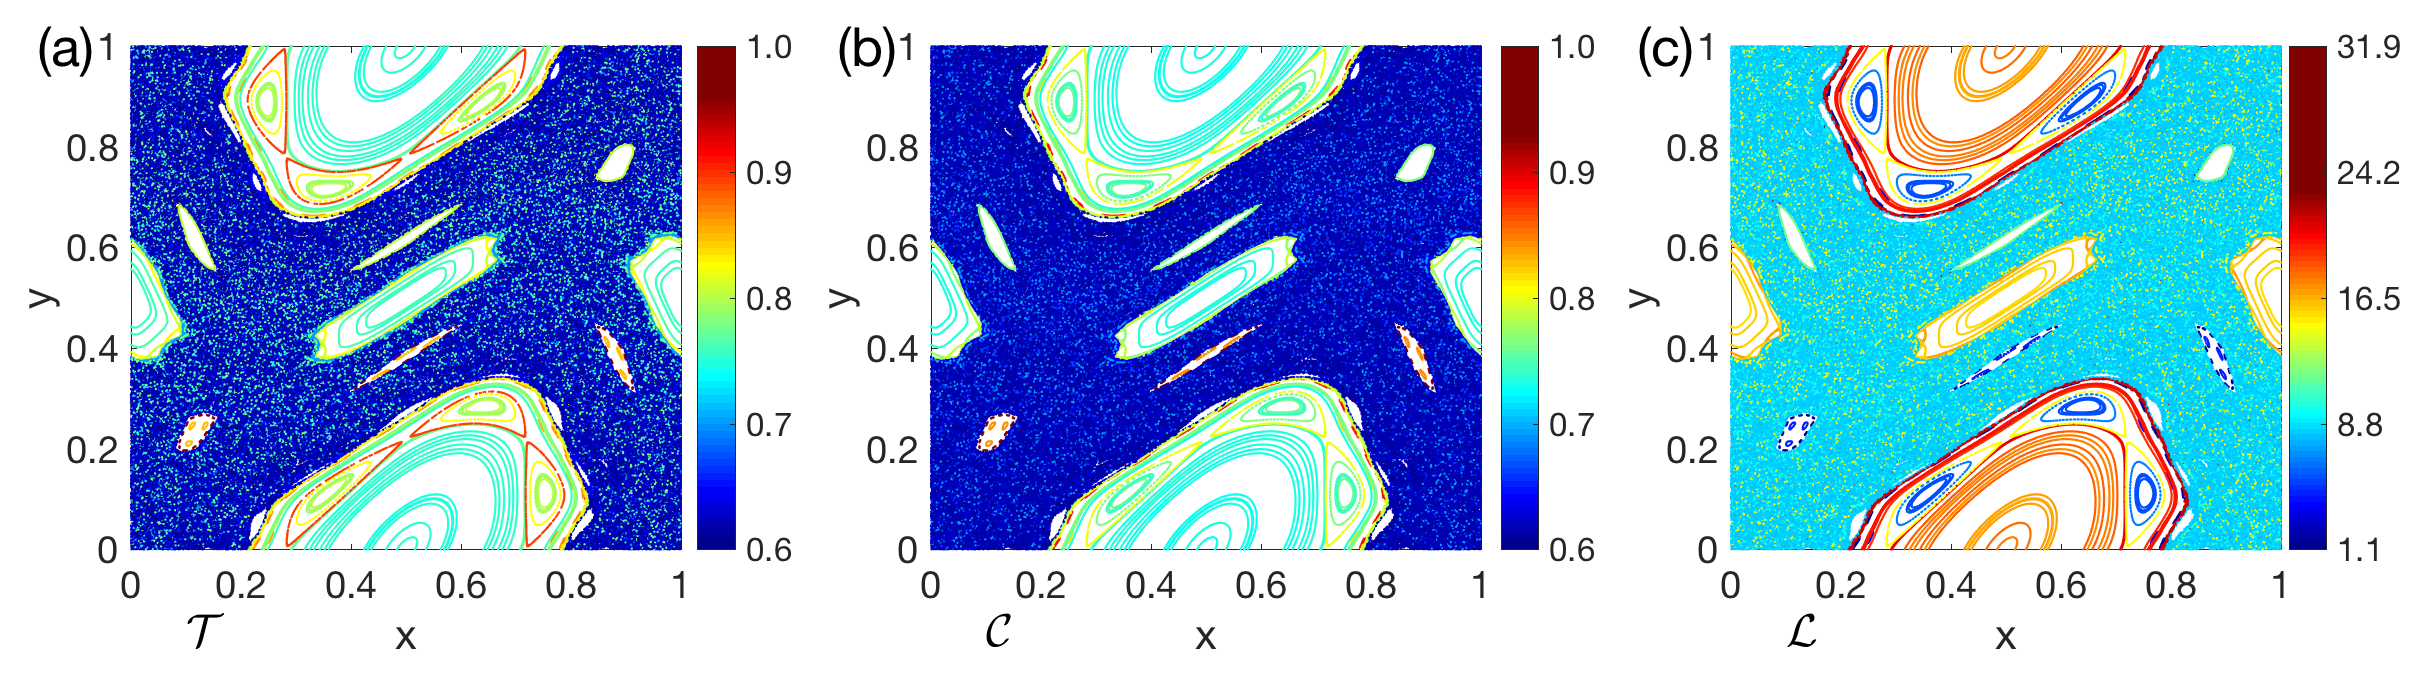
\includegraphics[width=\columnwidth]{Chapter07_Applications/stdFixedRRP.eps}
\caption{\small {Phase space of the standard map (Eq.~\eqref{std_map_book}) characterized by recurrence statistics for the standard map using fixed $RR=0.02$. (a) $\mathcal{T}$, (b) $\mathcal{C}$, (c) $\mathcal{L}$. Reproduced from \cite{Zou2016d}. } \label{fig:sm_rec_rr}}
\end{figure}
		
		The overall structure of the phase space with its intermingled regular and irregular components is captured by all these RN measures as shown in Figs. \ref{fig:sm_rec_rr}.  Further dynamic  and geometric measures are discussed in \cite{Zou2016d}. Specifically, quasi-periodic trajectories are characterized by larger values of network transitivity $\mathcal{T}$ and $\mathcal{C}$, while filling chaotic ones have smaller $\mathcal{T}$ and $\mathcal{C}$ (Fig. \ref{fig:sm_rec_rr}(a, b)). 
		
		Traditionally a chaotic orbit can fill the complete domain (as $t\to\infty$), regular ones are distinct and mutually nested, which results in the chaotic domain is often larger than the regular one. The RN measure $\mathcal{L}$ depends clearly on the size of the orbit. Therefore, the pattern of $\mathcal{L}$ (Fig. \ref{fig:sm_rec_rr}(c)) is influenced by thresholds. In turn, when fixing $RR$ the effect of different spatial distances on the estimated RN average path lengths $\mathcal{L}$ is essentially removed (Fig.~\ref{fig:sm_rec_rr}(c)). 
		
				
		\emph{Characterize non-stationary systems}
		While the aforementioned results have been obtained for stationary systems, i.e., independent realizations of the system at fixed parameter values, tracing temporal changes in dynamical complexity of non-stationary systems is another interesting field of application with numerous examples in the real-world. Using model systems with drifting parameters such as the Lorenz \cite{Donges2011} or R\"ossler systems, it is possible to systematically evaluate the performance of RN characteristics in a sliding windows framework, underlining their capabilities for discriminating between qualitatively different types of dynamics and different degrees of complexity in non-stationary (transient) runs as well. For the example of a linearly drifting control parameter $c$ of the R\"ossler system, we find that the values at which bifurcations between periodic and chaotic behavior occur in the non-stationary system do well coincide with the numerically estimated bifurcation points of the autonomous system inferred from, indicating that in the considered example, transient dynamics close to the bifurcation points does not play a major role as long as the considered RNs are still sufficiently large to obtain a reliable statistics. 
		
		There is another category of non-stationary process of long-term correlated stochastic dynamics, for instance, fractional Brownian motion (fBM) as we discussed in Sec. \ref{subsec:practicalRN}, which needs special care when applying recurrence based network analysis. In the case of non-stationary fBm, the fundamental concepts of phase space reconstruction and low-dimensional dynamics do not apply anymore \cite{Zou2015}. Therefore, the results presented in \cite{Liu2014} hold only for the particular choices of the algorithmic parameters (for instance, length of time series, embeddings etc), showing limited physical interpretations. One solution to the problem could be transforming the process in a way so that it becomes stationary \cite{Zou2015}. In recent applications to non-stationary real-world time series~\cite{Donges2011,Donges2011a}, the authors have removed non-stationarities in the mean by removing averages taken within sliding windows from the data. In the particular case of fBm, the underlying stochastic process can be transformed into a stationary one by a first-order difference filter, i.e., by considering its increments $x_{i+1}- x_i$. The transformed series is commonly referred to as fractional Gaussian noise (fGn) in analogy with the classical Brownian motion arising from an aggregation of Gaussian innovations. Notably, fGn retains the long-range correlations and Gaussian probability density function (PDF) from the underlying fBm process. 
		
		Because of its stationarity, for fGn the embedding parameters can be chosen more properly than for fBm. Following the discussion in Sec. \ref{subsec:practicalRN}, we choose embedding delay $\tau$ according to the autocorrelation function (ACF). In the case for $H < 0.5$ where $H$ is the Hurst exponent of the process, the estimated ACF drops to negative value at lag one resulting from subsequent values are negatively correlated for the anti-persistent process. Therefore, we choose $\tau = 1$ for $H < 0.5$. In contrast, for $H > 0.5$ we use the de-correlation time $\tau_{0.1}$ as an estimator for embedding delay $\tau$, which increases with rising $H$ as one would expect since larger $H$ indicates a longer temporal range of correlations. The embedding dimension $m$ is chosen via the FNN method. Unlike for fBm, our results suggest that the optimal value $m$ rises with an increasing length of the time series. In general, considerably higher values of $m$ are suggested than for fBm, which matches the theoretical expectations more closely. However, due to the finite sample size, we still find a vanishing FNN rate at a finite embedding dimension, which is probably related to a lack of proper neighbors when high dimensions are considered. 
				
		We have demonstrated in~\cite{Donner2011b} that the RN characteristics transitivity $\mathcal{T}$ and global clustering coefficient $\mathcal{C}$ provide relevant information for characterizing the geometry of the resulted RNs, which has been numerically supported for various deterministic-chaotic systems. Furthermore, the theory presented in \cite{Donges2012} shows that the corresponding considerations can be extended to any kind of process with a given state density $p(\mathbf{x})$. Here, we exemplify these considerations for the case of fGn and examine how the transitivity properties of RNs arising from such stationary long-range correlated stochastic processes depend on the characteristic Hurst exponent. From the numerical perspective, we show the dependence of the results on the embedding dimension $m$ explicitly. 
		\begin{figure}	
			\centering
			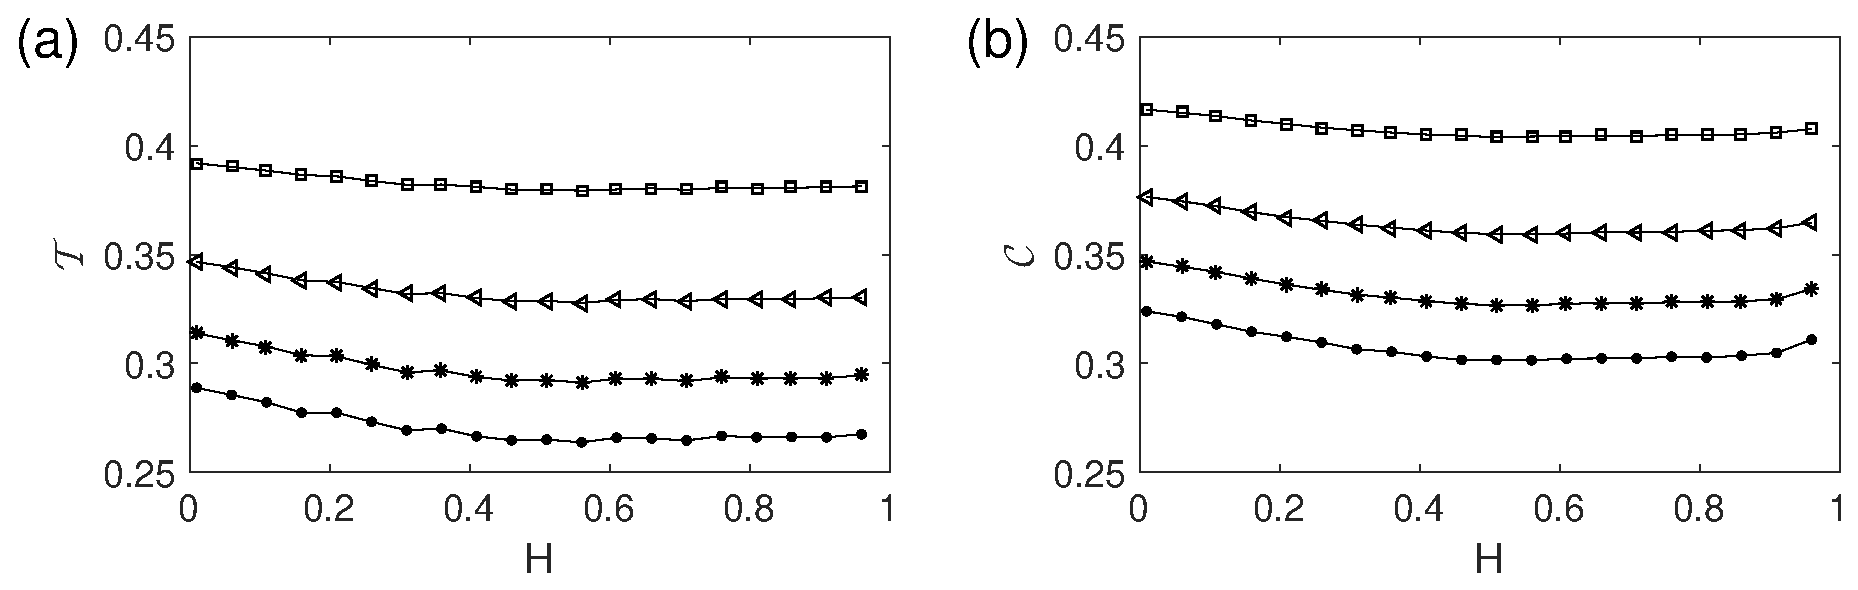
\includegraphics[width=\columnwidth]{Chapter07_Applications/netRec4DimiHP.eps}
		\caption{Dependence of (a) RN transitivity $\mathcal{T}$ and (b) global clustering coefficient $\mathcal{C}$ for fGn on the Hurst exponent $H$ for different embedding dimensions ($m=3$: $\square$, $m=4$: $\triangleleft$, $m=5$: $\ast$, $m=6$: $\bullet$), taken over 200 independent realizations and using a RN edge density of $\rho=0.03$. The embedding delay has been kept at the same value for all realizations with the same $H$ according to the de-correlation time $\tau_{0.1}$. In all cases, $N=2^{12}$. Reproduced from \cite{Zou2015}.  \label{fig:fgn_trans_H}}
\end{figure}
	
		For $H>0.5$, Fig.~\ref{fig:fgn_trans_H} shows that for a given embedding dimension $m$, both $\mathcal{T}$ and $\mathcal{C}$ do not depend on $H$, which is expected since the $m$-dimensional Gaussian PDF of the process does not depend on $H$ \cite{Donges2012,Zou2015}. Some minor deviation from the constant values can be observed at $H$ close to 1, i.e., close to the non-stationary limit case represented by $1/f$-noise, which might be due to numerical effects \cite{Zou2015}. 
		
		For $H<0.5$, both $\mathcal{T}$ and $\mathcal{C}$ rise with decreasing $H$. The reason for this behavior is that $\tau=1$ is the recommended, but still not ``optimal'' embedding delay for anti-persistent processes. Specifically, the closer $H$ approaches 0, the stronger is the anti-correlation at lag one. This means that with the same embedding delay $\tau=1$, the smaller $H$ the stronger are the mutual correlations between the different components of the embedding vector. As a consequence, the state vectors do not form a homogeneous $m$-dimensional Gaussian PDF with independent components in the reconstructed phase space, but are stretched and squeezed along certain directions, so that the resulting geometric structure appears significantly lower-dimensional than $m$. More numerical considerations have been discussed in \cite{Zou2015}, for instance, systematical biases when $H$ is close to $0$ and finite sample size $N$. 

		
		\emph{Characterize parameter space} 
		In order to illustrate the performance of RN transitivity ${\mathcal{T}}$ and average path length ${\mathcal{L}}$ as tracers for qualitative changes in the dynamics of complex systems, we briefly recall results originally obtained by the authors \cite{Zou2010}. In the latter work, the RN properties have been successfully used to discriminate between periodic and chaotic solutions in a two-dimensional subspace of the R\"ossler system. As Fig.~\ref{fig:roessler_shrimp} reveals, there are sequences of transitions between periodic and chaotic solutions. Specifically, we clearly see from the figure that the periodic windows are characterized by higher values of ${\mathcal{T}}$ and ${\mathcal{L}}$ than the chaotic solutions, which is in agreement with the general considerations discussed above. Specifically, for the periodic windows, we find $\hat{\mathcal{T}}$ close to $0.75$, the theoretical value for periodic dynamics (i.e., a system with effective dimension of $1$).
		\begin{figure}
		\centering
			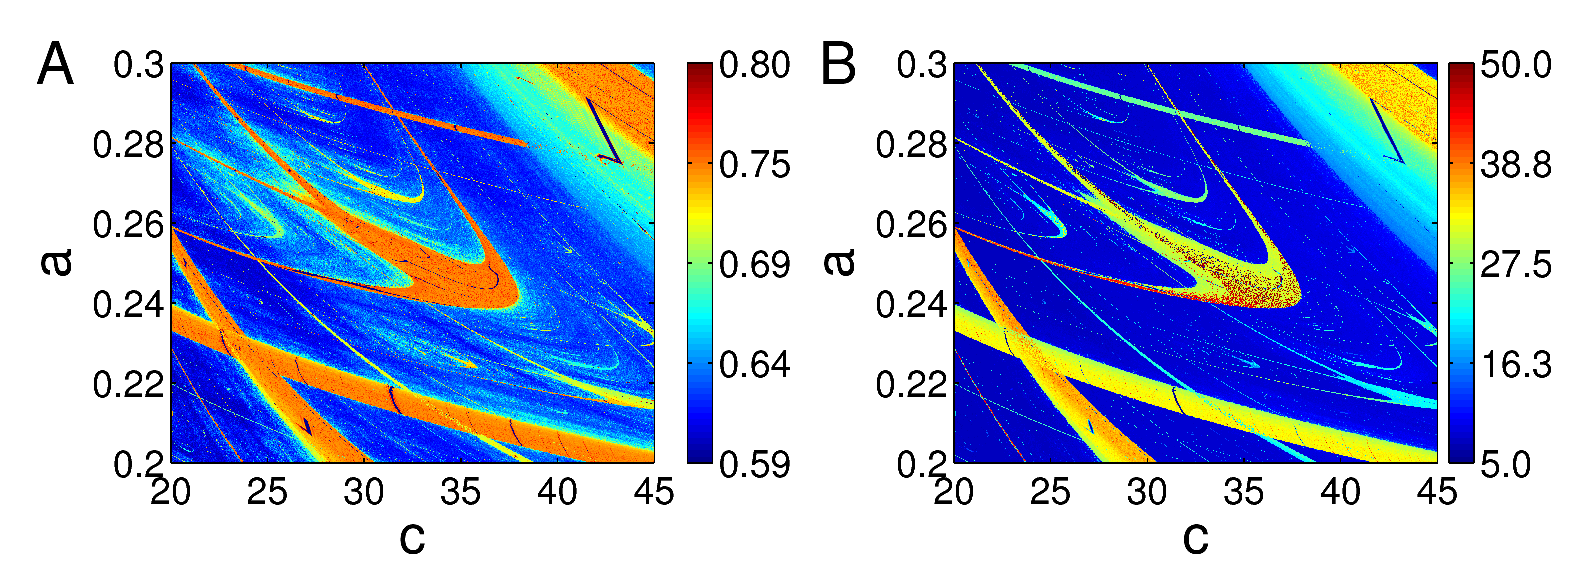
\includegraphics[width=\columnwidth]{Chapter07_Applications/ros_shrimp_eBook.eps} 
\caption{RN transitivity $\hat{\mathcal{T}}$ (A) and average path length $\hat{\mathcal{L}}$ (B) for a two-dimensional intersection ($a=b$) of the three-dimensional parameter space of the R\"ossler system (Eq.~\ref{eq:roessler}), displaying ``shrimp'' structures (i.e., self-similar periodic windows with complex shape). For details, see~\cite{Zou2010}.}
\label{fig:roessler_shrimp}
\end{figure}

		In a similar way, we may use the RN framework for capturing the signatures of qualitative changes in the attractor's shape and invariant density as a single control parameter is varied systematically. In a previous study using the R\"ossler system, we have investigated the RN properties across the transition from the classical phase-coherent R\"ossler attractor to the non-coherent funnel regime \cite{Zou2012c}. Our results indicate that phase coherence -- in a similar spirit as fractal dimension -- should be characterized from a geometric rather than a dynamics viewpoint. However, as of today there is no single RN-based index for phase coherence that has been explicitly derived from theoretical considerations.
		
		
		\todo[inline]{coupling directions and synchronization analysis.}

		\subsubsection{Real-world applications}
		Although much recent work on RNs and multivariate generalizations thereof has been focused on the development of the theoretical framework and its numerical exploration using simple low-dimensional model systems, there have already been some first successful applications to characterizing system's properties from experimental or observational time series. For example, the successful application of RN to predict protein structural classes has been reported in \cite{Olyaee2016}. 
		
		{\color{red} As Norbert suggested, we need 1-2 explicit examples showing the applications in this subsection. Please make suggestions. }
		
		\emph{Applications in climatology: }
		One important field of recent applications is paleoclimatology, which has already been taken as an illustrative example in the seminal paper by Marwan \textit{et~al.} \cite{Marwan2009}. The corresponding study was later extended to some systematic investigation of the temporal variability profile of RN-based complexity measures for three marine sediment records of terrigenous dust flux off Africa during the last 5 million years. Donges \textit{et~al.} \cite{Donges2011} argued that RNs can be used for characterizing dynamics from non-uniformly sampled or age-uncertain data, since this methodological approach does not make explicit use of time information. In turn, due to the necessity of using time-delay embedding, there is implicit time information entering the analysis, which has been recognized but widely neglected in previous works. Notably, disregarding age uncertainty and sampling heterogeneity appears a reasonable approximation only in cases where the distribution of instantaneous sampling rates remains acceptably narrow. 

		The results of Donges \textit{et~al.} \cite{Donges2011a} pointed to the existence of spatially coherent changes in the long-term variability of environmental conditions over Africa, which have probably influenced the evolution of human ancestor species. Specifically, RN transitivity and average path length have been interpreted as indicators for ``climate regularity'' (i.e., the complexity of fluctuations as captured by the transitivity dimensions) and ``abrupt dynamical changes'', respectively. By identifying three time intervals with consistent changes of the RN properties obtained from spatially widely separated records, it has been possible to attribute the corresponding long-term changes in the dynamics to periods characterized by known or speculated mechanisms for large-scale climate shifts such as changes in the Indian ocean circulation patterns, the intensification of the atmospheric Walker circulation, or changes in the dominant periodicity of Northern hemispheric glacial cycles. Moreover, Donges \textit{et~al.} \cite{Donges2011} demonstrated a good robustness of the results of RN analysis obtained in a sliding windows framework when varying the corresponding parameters (e.g., window size or embedding delay) over a reasonable range.

		As another methodological step towards better understanding climatic mechanisms, we have used two speleothem records for studying interdependencies between the two main branches of the Asian summer monsoon (the Indian and East Asian summer monsoon) by means of inter-system recurrence network approaches \cite{Feldhoff2012}. For this purpose, they selected two data sets of oxygen isotope anomalies from speleothems obtained from two caves in China and the Oman, respectively, which can be considered as proxies for the annual precipitation and, hence, the overall strength of the two monsoon branches over the last about 10,000 years. The asymmetries of the IRN cross-transitivities and global cross-clustering coefficients provided clear evidence for a marked influence of the Indian summer monsoon on the East Asian branch rather than vice versa, which is in good agreement with existing climatological theories. As a subsequent extension of this work, we emphasize the possibility of repeating the same kind of analysis in a sliding windows framework, thereby gaining information on possible temporal changes of the associated climatic patterns during certain time periods as recently revealed using correlation-based complex network analysis applied to a larger set of speleothem records from the Asian monsoon domain \cite{Rehfeld2012}.

		In order to characterize dynamical complexity associated with more recent environmental variability, Lange and B\"ose \cite{Boese2012,Lange2013Book} used RQA as well as RN analysis for studying global photosynthetic activity from remote sensing data in conjunction with global precipitation patterns. Specifically, they studied 14-years long time series (1998-2011) of the fraction of absorbed photosynthetically active radiation with a spatial resolution of 0.5$^o$ around the Earth and a temporal sampling of about ten days, providing time series of $N=504$ data points. Their results revealed very interesting spatial complexity patterns, which have been largely, but not exclusively determined by the amplitude of the annual cycle of vegetation growth in different ecosystems.


		\emph{Applications in fluid dynamics: }
		In a series of papers, Gao \textit{et~al.} investigated the emerging complexity of dynamical patterns in two-phase gas-liquid or oil-water flows in different configurations using RN techniques. In general, multiple sensors measuring fluctuations of electrical conductance have been used for obtaining signals that are characteristic for the different flow patterns. For gas-liquid two-phase upward flows in vertical pipes, different types of complex networks generated from observational data have been proposed, among which the degree correlations (assortativity) of RNs was proven to be particularly useful for distinguishing between qualitatively different flow types \cite{Gao2009,Gao2009a,Gao2010a}. One may also construct a directed weighted RN \cite{Gao2012,Gao2012a,Gao2013b,Gao2013d,Zhang2013b}. For oil-water two-phase upward flows in a similar configuration, the global clustering coefficient of RNs reveals a marked increase in dynamical complexity (detectable in terms of a decreasing $\hat{\mathcal{C}}$) as the flow pattern changes from slug flow over coarse to very finely dispersed bubble flow \cite{Gao2013,Gao2013c}. In case of oil-water two-phase flows in inclined pipes \cite{Gao2010}, the motif distributions of RNs (specifically, the frequency distributions of small subgraphs containing exactly four vertices) revealed an increasing degree of heterogeneity, where the motif ranking was conserved in all experimental conditions, whereas the absolute motif frequency dramatically changed. The corresponding results were independently confirmed using some classical measures of complexity, which indicated increasing complexity in conjunction with increasing heterogeneity of the RN motif distributions. Finally, for characterizing horizontal oil-water flows \cite{Gao2013d}, RN and inter-system RN analysis were combined for studying conductance signals from multiple sensors. Specifically, cross-transitivity was found a useful measure for tracing the transitions between stable stratified and unstable states associated with the formation of droplets. Furthermore, Gao {\textit{et al.}} \cite{Gao2015a,Gao2016,Gao2016b,Gao2016c} further extended these ideas to construct multivariate weighted recurrences networks from multi-channel measurements from different oil-water flow patterns. 
		

		\emph{Applications in electrochemistry: }
		Zou \textit{et~al.} \cite{Zou2012b} studied the complexity of experimental electrochemical oscillations as one control parameter of the experiments (temperature) was systematically varied. By utilizing a multitude of complementary RN characteristics, they could demonstrate a systematic rise in dynamical complexity as temperature increased, but an absence of a previously speculated phase transition \cite{Wickramasinghe2010} separating phase-coherent from noncoherent chaotic oscillations. The latter results were independently confirmed using other classical indicators for phase coherence, as well as studies of a corresponding mathematical model of the specific electrochemical processes.


		\emph{Applications in medicine: }
		Finally, there have been a couple of successful applications in a medical context. Marwan \textit{et~al.} \cite{Marwan2010c} demonstrated that the global clustering coefficients of RNs obtained from heartbeat intervals, diastolic and systolic blood pressure allowed a reliable identification of patients with pre-eclampsia, a cardiovascular disease during pregnancy with a high risk of fetal and maternal morbidity. Their results were further improved by Ram\'{i}rez \textit{et~al.} \cite{Ramirez2012,Ramirez2013} who considered combinations of various RN-based network characteristics. In a similar spirit as for cardiovascular diseases, recent results point to the capability of RN characteristics for discriminating between the EEG signals of healthy and epileptic patients \cite{Subramaniyam2013}.

%		\subsubsection{Example I: palaeoclimate data}
%		\subsubsection{Example II: soil water }

	\subsection{Visibility graphs} \label{sec:appVGs}
	(H)VGs approaches have been applied so far for studying energy dissipation rates in fully developed turbulence \cite{Liu2010,Manshour2015,Manshour2015a}, financial data \cite{Ni2009,Yang2009,Qian2010}, physiological time series \cite{Lacasa2009,Shao2010,Dong2010,Ahmadlou2010,Jiang2013,Hou2014}, seizure detections by EEG signals \cite{Bhaduri2015,Liu2017a,Zhang2018}, cardiorespiratory interaction signals \cite{Long2014}, alcoholism identification by EEG signals\cite{Zhu2014}. In the geoscientific context, \cite{Elsner2009} studied the time series of annual US landfalling hurricane counts. Subsequently, \cite{Tang2010} presented a study on daily streamflow series from the US and China. VGs analysis has been reported in air temperature data from China \cite{Wang2009}, wind speed records from central Argentina \cite{Pierini2012}, quarterly macroeconomic series of China \cite{Wang2012}. {\emph{Telesca et al.}}\cite{Telesca2012} used VGs for studying seismic activity in Italy, and Corinth rift in western central Greece \cite{Hloupis2017}. Nonlinear features of seismic time series have been recently reviewed in \cite{Telesca2018b}. Both $k$ nearest neighbors network and VGs analysis show almost the same qualitative behavior and allow to reveal the underlying system dynamics in turbulent heated jets \cite{Charakopoulos2014}. Motif structures and subgraphs of VGs have been used to human ventricular fibrillation (ECG) time series \cite{Li2011,Li2012}, ECG diagnosis of epilepsy \cite{Tang2013},  air traffic flow data \cite{Liu2018}. Simple topological measures such as the diameter, average path length, modularity, clustering coefficient, density and hierarchical organizations of networks have been used to characterize different dynamic properties between atmospheric and oceanic variables \cite{CHARAKOPOULOS2018}. In addition, the (H)VGs have been proposed to predict catastrophes of a non-autonomous network which derived from a marine system \cite{Zhang2018b}, which demonstrates that the topological characteristics like average degrees of the networks do show pronounced signatures at the onset of catastrophes. Fractal characteristics of (H)VGs have been reported in fractional Brownian motions, which has been recently extended to multiparticle emission data in high energy heavy-ion collisions \cite{Mali2018}, which shows consistent power law degree distributions as compared to the results as obtained by the traditional sandbox algorithm. In \cite{Gao2016}, a slight modification of HVG algorithm has been proposed to extract the multiscale properties of time series from oil-water two phase flow signals. In the case of intermittent time series, some phenomenology theories have been obtained in order to link the laminar episodes and chaotic bursts with the connectivity of the resulting HVGs \cite{Nunez2013,Nunez2014}. 
	
	Here, we illustrate two specific examples showing the applications of (H)VG analysis to time series of sunspots. 				
		\subsubsection{Example I: sunspot numbers} \label{subsec:sunnum}
		Solar activity is characterized by complex dynamics superimposed to an almost periodic, about 11 years cycle. Zou {\textit{et al.}} \cite{Zou2014a} performed the VGs analysis on both the daily and monthly sunspot series. The natural VGs focus on the effects of the local maxima on the resulting graphs. In order to disclose the contributions of local minima to the VGs, they proposed two ways to construct the network: one is from the original observable measurements and the other is from a negative-inverse-transformed series. In the particular case of sunspot series, local minima play important roles in forming the increasing and decreasing phases of the solar cycles. In \cite{Zou2014a}, they found that the degree distribution of the derived networks for the strong maxima has clear non-Gaussian properties, while the degree distribution for minima is bimodal. 
		
		Here, let us construct VGs for both the International Sunspot Number (ISN)~\cite{sidcDataBelgium} (see \cite{Zou2014a} for more consistent results that are based on the sunspot area (SSA) series). We perform VG analysis for both monthly and daily sunspot series, which yields, respectively, month-to-month and day-to-day correlation patterns of the sunspot activities. The degree sequence $k_i = \sum_j A_{i,j}$ reflects the maximal visibility of the corresponding observation in comparison with its neighbors in the time series. Furthermore, the degree distribution is denoted as $p(k)$. In the case of sunspot time series, one is often required to investigate what contributions local minimum values make to the network -- something that has been largely overlooked by the traditional VGs. One simple solution is to study the negatively inverted counterpart of the original time series, namely, $-x(t_i)$, which quantifies the properties of the local minima. We use $k_{-x}$ and $p(k_{-x})$ to denote the case of $-x(t_i)$. Here, we remark that this simple inversion of the time series allows us to create an entirely different complex network. 
		
		Figure~\ref{sn_sa_data}(a,b) show the degree distributions $p(k)$ of the VGs derived from the ISN $x(t_i)$ with heavy-tails corresponding to hubs of the graph, which clearly deviates from Gaussian properties. In contrast, $p(k_{-x})$ of the negatively inverted sunspot series $-x(t_i)$ shows a completely different distribution, consisting of a bimodal property (Figure~\ref{sn_sa_data}c,d), extra large degrees are at least two orders of magnitude larger than most of the vertices (Figure~\ref{sn_sa_data}(d)).
		\begin{figure}
  		\centering
			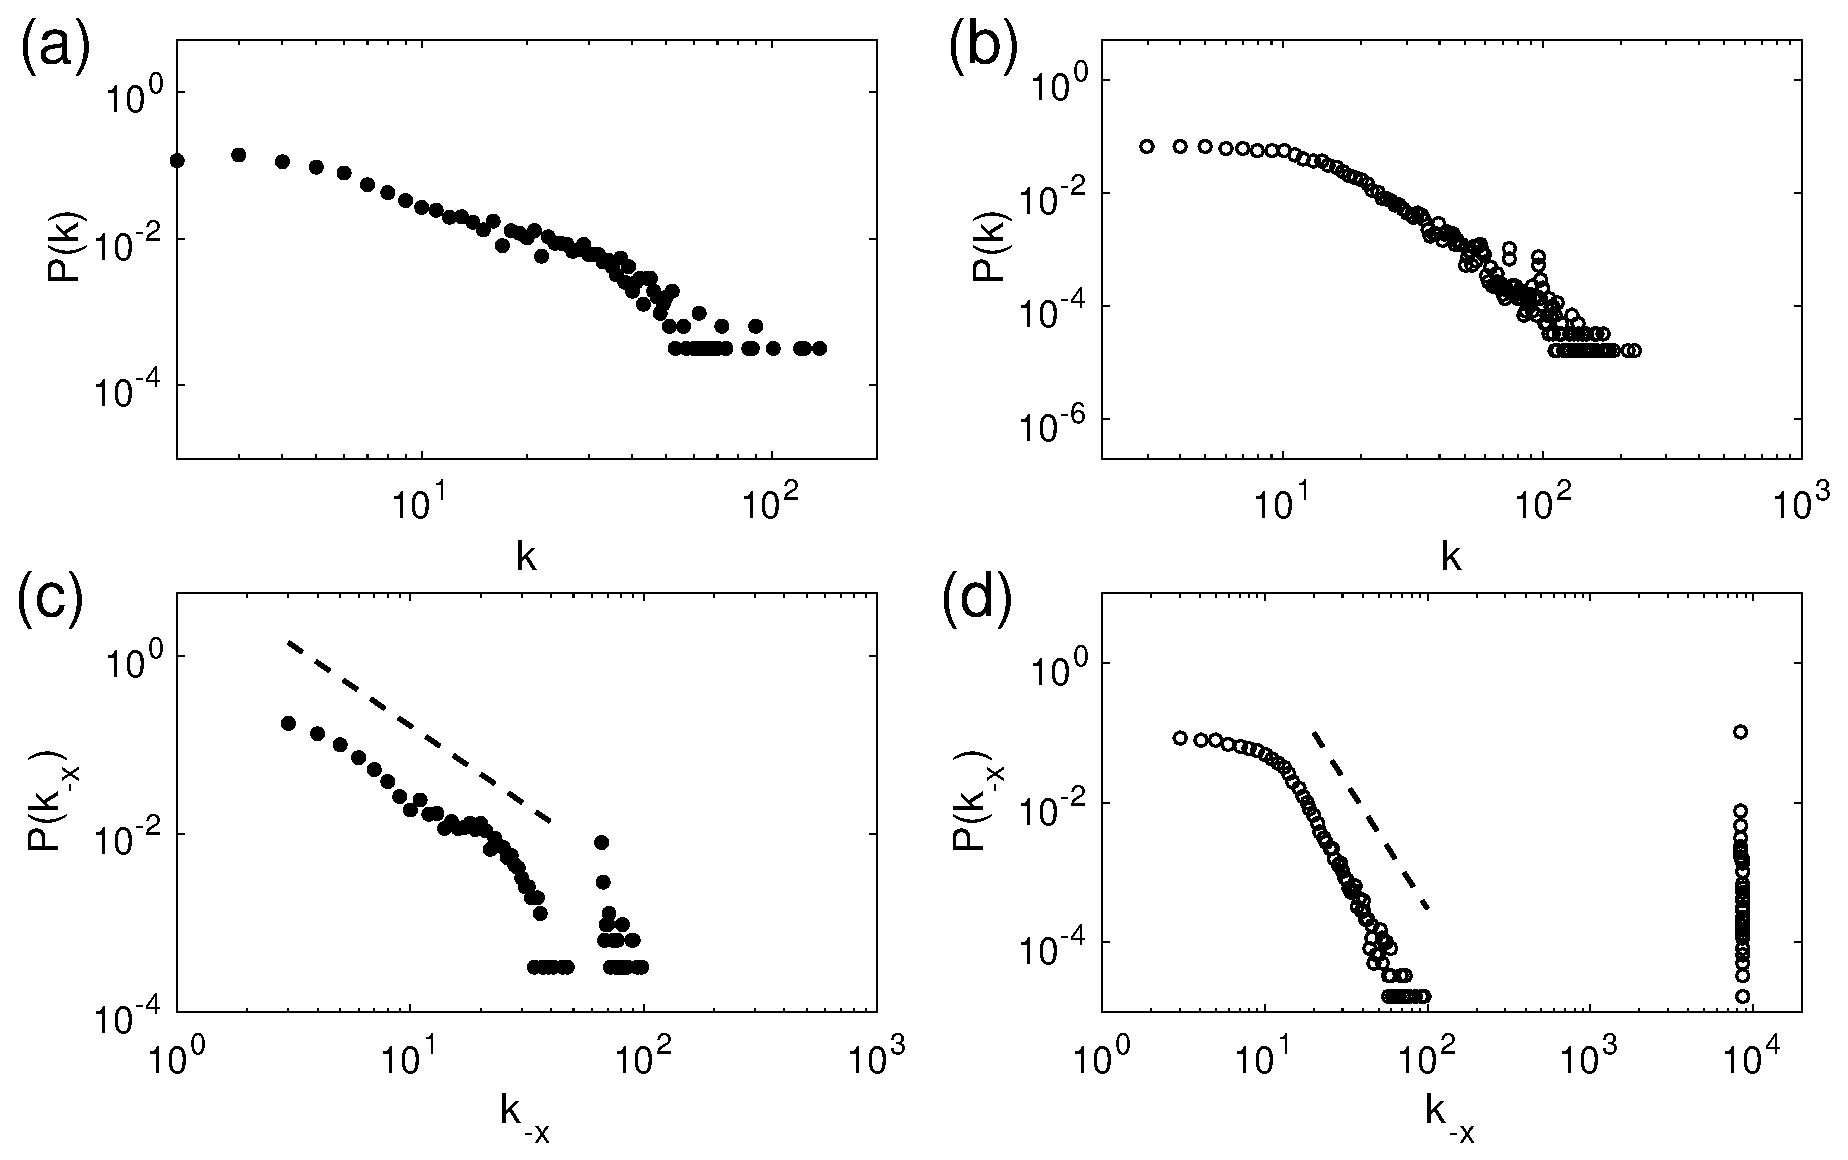
\includegraphics[width=0.8\columnwidth]{Chapter07_Applications/pdf_degreeBelgimN.eps}
		\caption{Degree distribution $p(k)$ of VGs from monthly (a,c) and daily data (b,d). (a,b) is for $x(t_i)$, and (c,d) $-x(t_i)$. One would suspect a fit to the first part of $p(k_{-x})$ yields that the slope of dashed line in (c) is 1.79, and that of (d) is 3.61, {\emph{but}} all $p$-values are $0$, rejecting the hypothetical power laws.} \label{sn_sa_data}
		\end{figure}	
		Since well-defined scaling regimes are absent in either $p(k)$ or $p(k_{-x})$ (nor do they appear in the cumulative distributions, see more details of the statistical tests in \cite{Zou2014a}), we may reject the hypothetical power laws. 
		
		Based on the degree sequences $k_x$ and $k_{-x}$, Zou {\textit {et al.}} \cite{Zou2014a} further investigated the long term variations of local maxima/minima of the sunspot series.  They found that the positions of strong maxima are largely homogeneously distributed over the time domain, while that of the strong minima are much more clustered in the time axis. This suggests that the strong active regions of sunspots appear more or less independently of each other, in contrast, the process of the strong minima has a positive long term correlation. The hidden regularity of the time positions of maxima/minima has been characterized by the waiting time distribution: the interval between two successive events is called the waiting-time. The distribution of the waiting time between two subsequent maxima sunspot deviates significantly from an exponential function \cite{Zou2014a}. In contrast, the waiting times between subsequent strong minima have a power-law distribution where a statistically significant scaling regime has been found. These results of the difference between maxima and minima could be used for evaluating models for solar activity because they reflect important properties that are not included in other measures reported in the literature.
		
		VGs for sunspot series show rich community structures, each of which mainly consists of the temporal information of two consecutive solar cycles. The solar cycle of approximately 11-years yields that most of the temporal points of the decreasing phase of one solar cycle are connected to those points of the increasing phase of the next cycle in the resulting VGs \cite{Zou2014a}. When the sunspot number reaches a stronger but more infrequent extreme maximum, we have inter-community connections, since they have a better visibility contact with more neighbors than other time points -- hence, forming hubs in the graph. The inter-community connections extend over several consecutive solar cycles encompassing the temporal cycle-to-cycle information. In Fig.~\ref{year_sspnDegBet}(a), we highlight some hubs of large degrees ($k_i > 15$), which have been suggested to identify solar cycles~\cite{Zou2014a}. In addition, there are strong positive correlations between large degrees $k_i$ and high betweenness $b_i$, which further characterizes the node's ability to transport information from one place to another along the shortest path as shown in Fig.~\ref{year_sspnDegBet}(b). 
		\begin{figure}
  		\centering
   			\includegraphics[width=\columnwidth]{Chapter07_Applications/network261_degree_between.eps}
			\caption{Network representations of the VG constructed from the annual sunspot numbers of the entire series. Highlighted visible nodes are: (A) large degrees ($k_i>15$), and (B) high betweenness centrality ($b_i>0.2$). } \label{year_sspnDegBet}
		\end{figure}


		\subsubsection{Example II: Asymmetry of sunspots} \label{subsec:sunspotsAsym}
		In the previous Sec. \ref{subsec:sunnum}, we performed (H)VG analysis for the sunspots series. In addition, in the line of this research, another important features of sunspots is the presence of a marked, time-varying hemispheric asymmetry, which have not yet been completely uncovered. The hemispheric asymmetry of solar activity manifests itself in the statistical properties of a variety of activity indicators such as sunspot numbers, areas and spatial distribution, the numbers of flares and coronal mass ejections, solar radio and X-ray flux, etc., and has been recognized to vary on multi-decadal time scales (see, e.g.,\cite{Newton1955,Carbonell1993,zolotova2006,donner2007,donner2008a,Li2008MNRAS,li2008a,zolotova2009}, and references therein). Notably, it is commonly believed that the observed distinct hemispheric asymmetry is an intrinsic property associated with the underlying solar magnetic field dynamics, which in turn serves as the driver of solar activity responsible for particle and electromagnetic emissions directly affecting the Earth. Traditionally, the North--South asymmetry of solar activity has been mainly defined in terms of amplitude differences between the hemispheric values of different properties \cite{Newton1955}. Recently, it has been argued that phase information should be explicitly taken into account as well, noting that a mutual time shift between the activity cycles observed separately at both solar hemispheres could provide a significant contribution to the observed asymmetry \cite{zolotova2006,donner2007}. However, even despite these methodological advances, properly quantifying the North--South asymmetry is a challenging problem by itself. Specifically, the complex dynamics of the entire solar activity cycles calls for replacing traditional linear statistical approaches by methods originated in the field of nonlinear dynamics.

		In \cite{Zou2014}, Zou {\textit{et. al}} proposed (H)VGs analysis to study the asymmetric distributions of the sunspots over the solar surface. They have argued that both VGs and HVGs provide complementary information on hemispheric asymmetries in dynamical properties. More specifically as we discussed in Sec. \ref{subsec:jointdegreeVG}, the excess degree $\Delta k(t)$ (Eq. \eqref{eq:deltaK}) and the relative excess degree $\Delta_{rel} k(t)$ (Eq. \eqref{eq:deltaReK}) have been proposed to characterize the possible asymmetric properties for (H)VGs that are reconstructed from bivariate time series, which resulted two interacting layers $\alpha$ and $\beta$. These two measures are based on the computations of joint degree $k^{joint}(t)$ (Eq. \ref{eq:jointK}) and the conditional degree sequences $k_{{[\alpha]}, {[\beta]}}^{O}(t)$ (Eq. \ref{eq:nad}). Here we review some results based on $\Delta k(t)$ and $\Delta_{rel} k(t)$ and some more details are retrieved in \cite{Zou2014}. We emphasize that the absolute excess degree can be easily interpreted in terms of inter-hemispheric differences, whereas the relative excess degree partially corrects for the skewness effect and allows quantitatively assessing the relevance of differences between the degree sequences of both hemispheres.

		First we construct the (H)VGs for monthly hemispheric sunspot area series $A_{N}(t)$ and $A_{S}(t)$, yielding the degree sequences $k_\mathrm{N}(t)$ and $k_\mathrm{S}(t)$, respectively. The about 11~years solar activity cycle will be clearly visible in the degree sequences and, hence, the joint and conditional degree sequences. Therefore in \cite{Zou2014}, the long-term asymmetric distribution behavior of the sunspots has been captured by utilizing a sliding window technique that averages the degree sequence over some time period. In all following considerations the window size has been chosen as $w = 270$ months, with a mutual overlap of 12 months between subsequent time windows. This specific choice of the window size covers about one full period of the solar magnetic field polarity cycle (approximately 22 years). Note that there are no marked changes in the long-term variability of the (H)VG-based characteristics for $w$ being between about 180 and 400 months.
\begin{figure}
	\centering
	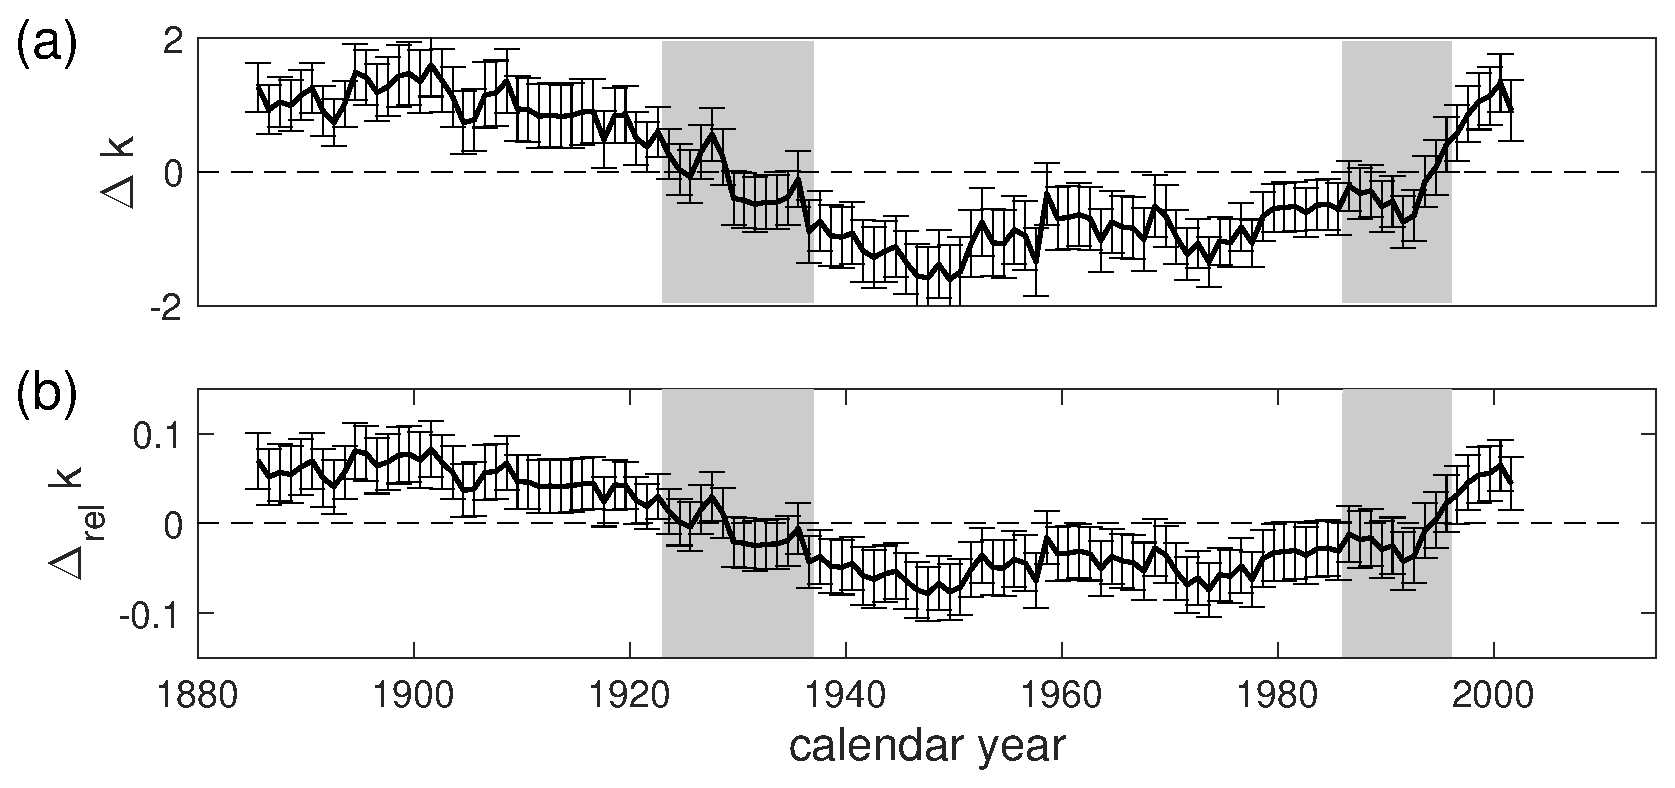
\includegraphics[width=0.8\columnwidth]{Chapter07_Applications/north_southDegreeComXWin130P.eps}
\caption{\small {(a) absolute and (b) relative excess degrees obtained from the VGs of $A_{N,S}$ computed over the sliding windows with a width of $w = 270$ months and a mutual overlap of $12$ months. Error bars display mean values and standard deviations within a given time window centered at the respective point in time. Gray areas mark those time intervals where the sign of the excess degree changes. Reproduced from \cite{Zou2014}. }
\label{degreeComX_ns_area270}}
\end{figure}		
Figure \ref{degreeComX_ns_area270} shows the mean features associated with the degree sequences for our sliding windows, together with the associated window-wise standard deviations. Our results reveal two transitions between periods of positive and negative mean (absolute and relative) excess degrees, which take place at about 1925--1935 (from higher degrees in the Northern Hemisphere to those in the Southern one) and 1985--1995 (vice versa). Furthermore, positive (negative) excess degrees imply higher mean degrees in the Northern (Southern) Hemisphere. These observations have been partially explained by the strong asymmetry of the probability distributions of sunspots over the north and south hemispheres, for instance, very high positive skewness. Notably, absolute and relative excess degrees exhibit qualitatively the same long-term variability. 
		
\begin{figure}
	\centering
	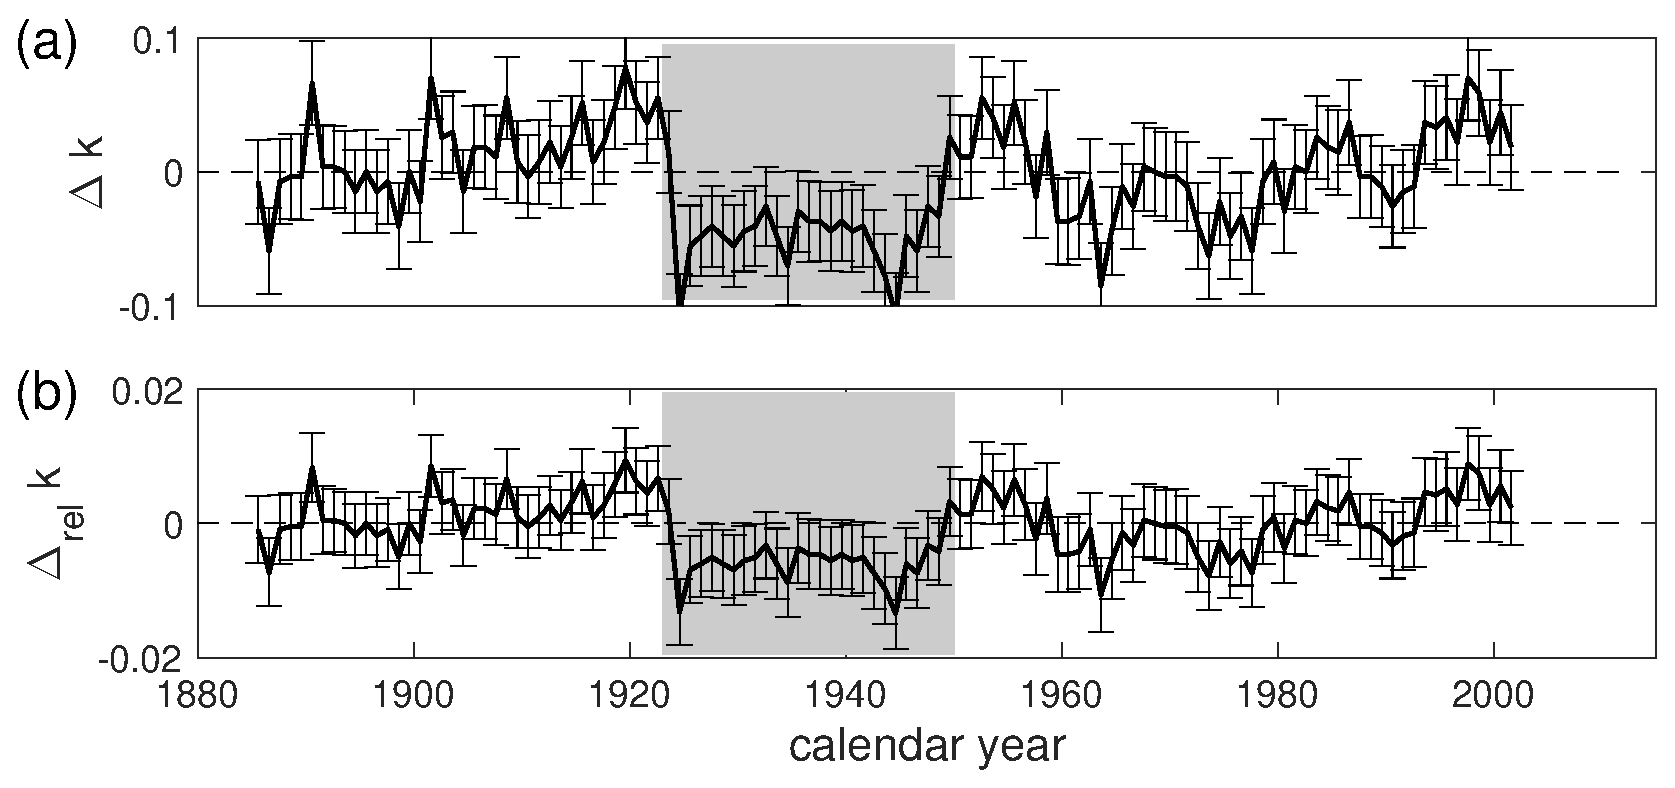
\includegraphics[width=0.9\columnwidth]{Chapter07_Applications/north_southDegreeComXWin130HVGP.eps}
\caption{\small {As in Fig.~\ref{degreeComX_ns_area270} for the corresponding HVG properties. The gray area indicates the only considerably long time interval with statistically significant hemispheric asymmetry of the mean conditional degree. Reproduced from \cite{Zou2014}. }
\label{HVG}}
\end{figure}		
		
		The corresponding analysis by mean of HVGs is shown in Figure \ref{HVG}, which reveals some interesting facts: first of all, all degree-related quantities obey considerably lower values and weaker overall variability than for the VG. This is to be expected since the HVG is a subgraph of the VG. However, while the absolute degree values in the HVG typically reduce by a factor of about 2--4 in comparison with the VG, the absolute excess degrees are by more than one order of magnitude smaller (Fig. \ref{HVG}). 

		Moreover, for the HVG-based excess degree $\Delta k(t)$ we do not find comparably clear indications for transitions between time periods with clear hemispheric predominance as for the VG (Fig. \ref{HVG}(a)). The only notable exception is the time period between about 1925 (corresponding to the formerly identified first transition in the VG) and 1950, where the excess degree of the HVG is significantly negative (as also observed before for the VG). Specifically, the transition in the hemispheric predominance reflected by the VGs' conditional degree sequences coincides with a sharp drop in the corresponding series for the HVG at about 1925, whereas the end of the period of significantly negative excess degrees in the HVG at about 1950 accompanies the termination of the gradual downward trend of the excess degree obtained from the VGs (Fig. \ref{HVG}(b)). Taken together, we interpret these findings such that the effect of the asymmetry of the hemispheric sunspot area values mostly dominates possible variations in dynamical characteristics. However, to this end we tentatively conclude that parts of the observed long-term changes of the VG-based excess degree cannot be explained by combining the corresponding changes in skewness and HVG-based excess degree (i.e., distribution and dynamics, respectively). One possible reason for this could be complex changes in the PDF of the sunspot areas, which go beyond fluctuations in skewness, but yet have a significant effect on the resulting VGs' properties.
		
		In summary, we conclude that temporal changes in the hemispheric predominance of the graph properties lag those directly associated with the total hemispheric sunspot areas. These findings open a new dynamical perspective on studying the North--South sunspot asymmetry, which needs to be further explored in future work. 


	\subsection{Transition networks}
	Depending on the particular symbolic representations of time series, there are various applications of transition network approaches to real time series. For instance, co-movement time series of economic growth and high-end talent development efficiency \cite{Zhang2018b}. Here we focus on the application of ordinal pattern transition network approach as proposed by McCullough {\textit{et al.}} in \cite{McCullough2015}, where they applied this analysis to experimental time series generated by a diode resonator circuits. They argue that the network size, mean shortest path length, and network diameter are highly sensitive to the interior crisis captured in this particular data set. Meanwhile, the ordinal pattern partition networks have been reconstruct from Electrocardiogram (ECG) data from patients with a variety of heart conditions \cite{Kulp2016b}. Network measures of mean degrees, entropies of the set of ordinal patterns and the number of non-occurring ordinal patterns have been computed for the resulting transition networks, showing statistically significant difference between healthy patients and several groups of unhealthy patients with varying heart conditions. 
	
	In \cite{McCullough2017b}, McCullough {\textit{et al}} have introduced to compute both local and global out-link entropies of ordinal transition networks to quantify the complexity of temporal structure in the networks from time series. The numerical comparative investigation in the R\"ossler system has demonstrated that these complexity measures track dynamical changes through period doubling and periodic windows over a range of the bifurcation parameter. Furthermore, the analysis has been applied to time series of electrocardiograms (ECGs). More specifically, complexity measures are able to capture the unique properties, discriminating between short-time ECG recordings characterized by normal sinus rhythm(NSR), ventricular tachycardia (VT) and ventricular fibrillation (VF). The global node out-link entropy of each time series is computed for both a short and a long time embedding lag and the resulting two-dimensional vector constitutes a measure of multiscale complexity description. In addition, the ordinal network analysis is performed to characterize age-related effects in interbeat interval dynamics from ECGs. 
		
	Another application of ordinal transition network method is to characterize synchronization transitions. In \cite{Zhang2017b}, they proposed to construct ordinal pattern partition transition networks for multivariate time series. This approach has been demonstrated to be useful for identifying dynamical regimes shifts and characterizing routes to phase synchronization. In particular, they consider three diffusively coupled R\"ossler systems via $x$ component \cite{Nawrath2010}, which read
\begin{equation} \label{threeRosPRL}
\left ( \begin{aligned}
& \dot{x}_k \\ 
& \dot{y}_k \\
& \dot{z}_k
\end{aligned} \right )
= \left ( \begin{aligned}
& -\omega_k y_k - z_k + \sum_{l\neq k} \kappa_{k,l}(x_l - x_k) \\ 
& \omega_k x_k + 0.165 y_k \\
& 0.4 + z_k(x_k - 8.5)
\end{aligned} \right ),
\end{equation}
where $k = 1, 2, 3$ and $\kappa$ is the coupling strength. We consider non-identical oscillators by choosing $\omega_1 = 0.98, \omega_2 = 1.02, \omega_3 = 1.06$. The oscillator $k = 2$ is bidirectionally coupled to both $k=1$ and $k=3$, whereas there is no direct coupling between $k=1$ and $k = 3$. The Eqs. \eqref{threeRosPRL} are numerically integrated by the fourth-order Runge Kutta method with integration step $h = 0.01$. We construct ordinal pattern transition networks from the $x_k$ components, namely, $(x_1, x_2, x_3)$ and the definitions of patterns have been summarized in Tab. \ref{tab:3D}. The results are shown in Fig. \ref{fig:rosslerSync}, which have been averaged over 50 random initial conditions when integrating Eqs. \eqref{threeRosPRL}. 

\begin{figure}[ht]
	\centering
	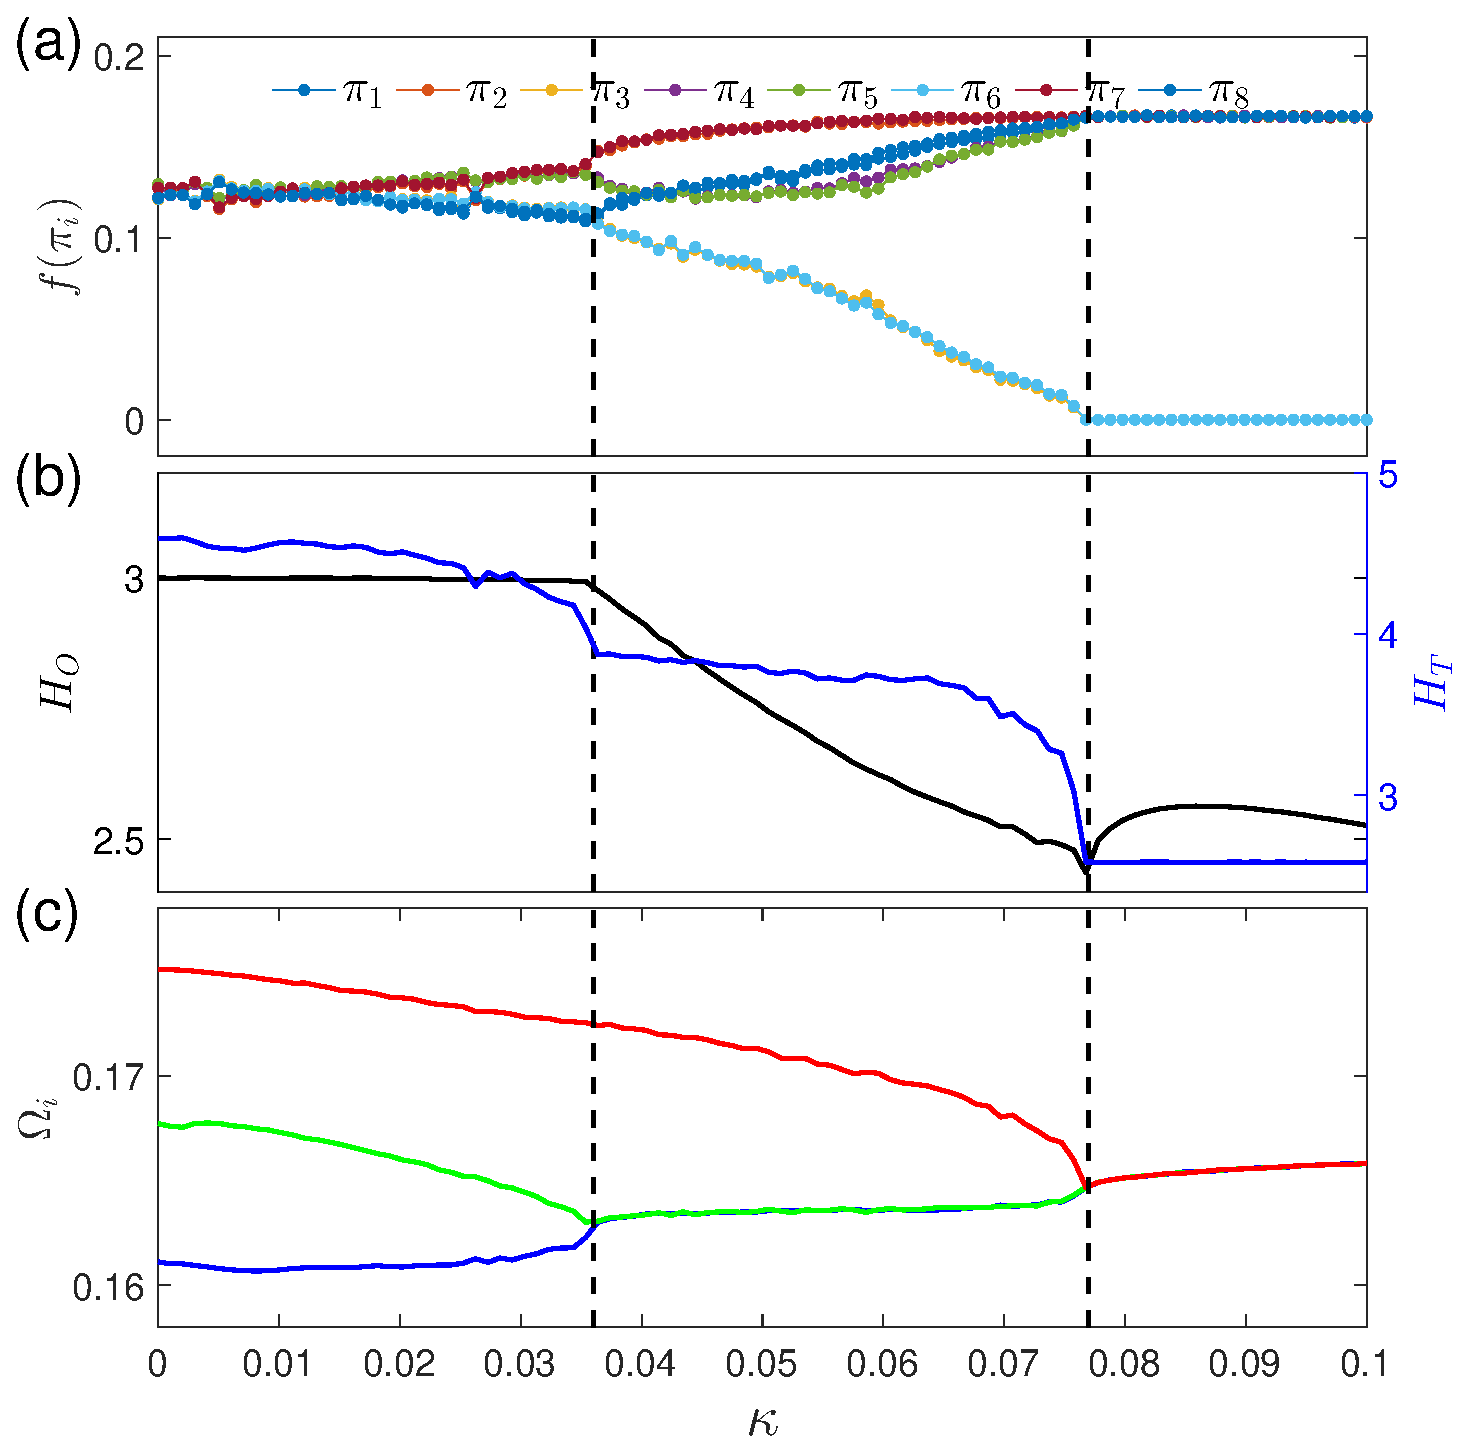
\includegraphics[width=0.6\columnwidth]{Chapter07_Applications/rosslerSync.eps}
\caption{Phase synchronization transitions of three coupled R\"ossler systems. (a) frequency of each ordinal pattern $f(\pi_i)$, (b) entropy values $\mathcal{H}_O$ (Eq. \eqref{eq:Ho}) and $\mathcal{H}_T$ (Eq. \eqref{eq:Ht}), (c) mean rotation frequency $\Omega_i$ of each oscillator. Subsystem $k_1$ and $k_2$ are synchronized at $\kappa_{c1}=0.036$, and $k_3$ joins the synchronization only at a stronger coupling strength $\kappa_{c2}=0.077$. Both critical coupling values are highlighted by vertical dashed lines. \label{fig:rosslerSync}}
\end{figure}

\begin{figure}[ht]
	\centering
	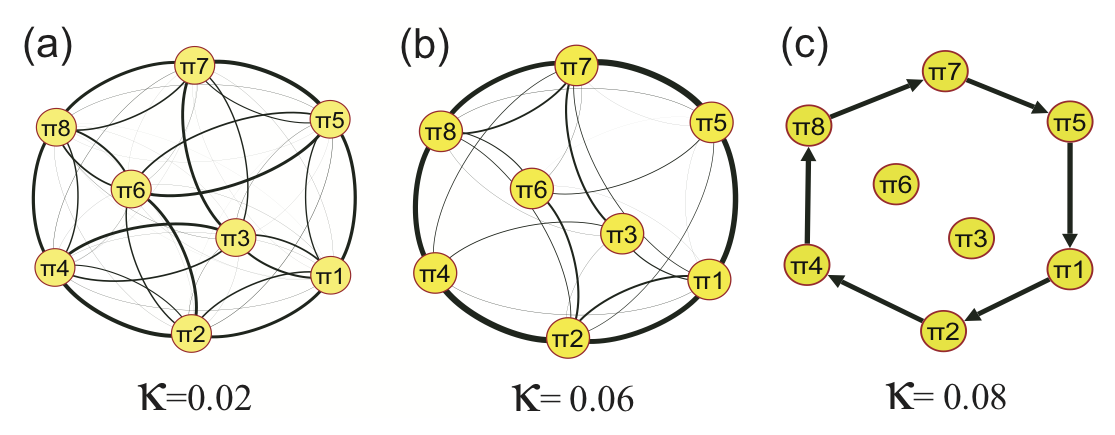
\includegraphics[width=0.7\columnwidth]{Chapter07_Applications/sync_net.eps}
\caption{Ordinal transition networks on the path to phase synchronization. (a) non-sync regime of $\kappa = 0.02 < \kappa_{c1}$, (b) oscillators $k=1$ and $k=2$ are phase synchronized, but not with $k=3$, $\kappa = 0.06 \in [\kappa_{c1}, \kappa_{c2}]$, (c) all three oscillators are phase locked $\kappa = 0.08 > \kappa_{c2}$. Thickness of links are determined by the transition frequencies. In (a) and (b), link arrows are suppressed. \label{fig:rosslerSyncNet}}
\end{figure}

In the regime of no synchrony ($\kappa < \kappa_{c1}=0.036$), three oscillators evolve almost independently such that all ordinal patterns have the same frequencies of $0.125$. There are rather small gradual changes only when $\kappa$ approaches to $\kappa_{c1}$ (Fig. \ref{fig:rosslerSync}(a)). The entropy value $\mathcal{H}_T$ is more sensitive to these gradual changes showing a pronounced decreasing trend, while $\mathcal{H}_O$ seems to be a constant (Fig. \ref{fig:rosslerSync}(b)). The average rotation frequencies $\Omega_k$ of each oscillator are shown in (Fig. \ref{fig:rosslerSync}(c)), which confirms no synchrony in this coupling regime.

In the regime that phase synchronization appears between oscillators $k=1$ and $k=2$, but not with $k=3$ ($\kappa \in [\kappa_{c1}, \kappa_{c2}] =[0.036, 0.077]$), we observe monotonic increasing trends for order patterns $\pi_1$, $\pi_2$, $\pi_7$, and $\pi_8$ (Fig. \ref{fig:rosslerSync}(a)). In addition, we find relatively slower increasing trends for patterns of $\pi_4$ and $\pi_5$. In contrast,  some monotonic decreasing trends are found for $\pi_3$ and $\pi_6$. The changes in the frequencies of order patterns are captured by both entropy values $\mathcal{H}_O$ and $\mathcal{H}_T$, showing gradual decreasing trends (Fig. \ref{fig:rosslerSync}(b)). The average rotation frequencies $\Omega_k$ are shown in Fig. \ref{fig:rosslerSync}(c), where $k=1$ and $k=2$ are phase locked to the same rotation frequency but not with $k=3$.

In the regime with all oscillators in phase synchronization ($\kappa > \kappa_{c2} = 0.077$), we find that frequencies of patterns $\pi_1$, $\pi_2$, $\pi_4$, $\pi_5$, $\pi_7$, $\pi_8$ converge to the same value $f(\pi_i) = 1/6$, while $\pi_3$ and $\pi_6$ are absent (Fig. \ref{fig:rosslerSync}(a)). In other words, forbidden patterns of $\pi_3$ and $\pi_6$ are observed if all oscillators are synchronized. The entropy $\mathcal{H}_O$ shows parabola-like trends (increasing first and then decreasing slowly), but $\mathcal{H}_T$ is a constant of $2.585$ (Fig. \ref{fig:rosslerSync}(b)). All mean rotation frequencies converge to the same value since three oscillators are phase locked (Fig. \ref{fig:rosslerSync}(c)).

In the process from non-synchrony to phase synchronization, the transition networks have experienced rather random transitions between all possible ordinal patterns to a state of transitions between a limited number of ordinal patterns as shown in Fig. \ref{fig:rosslerSyncNet}. In addition, we find $\pi_3$ and $\pi_6$ are forbidden patterns if all three oscillators are synchronized.

%	\subsection{Other approaches?}


